% FL-AV manuscript, IEEE two-column journal layout (IEEEtran).
% Build:  pdflatex paper && bibtex paper && pdflatex paper && pdflatex paper
% Figures: python paper/make_paper_figures.py --ieee   (writes paper/ieee/figures/)
\documentclass[journal]{IEEEtran}

\usepackage[T1]{fontenc}
\usepackage{times}
\usepackage[cmex10]{amsmath}
\usepackage{amssymb}
\usepackage{graphicx}
\usepackage{booktabs}
\usepackage{array}
\usepackage{multirow}

\usepackage{cite}
\usepackage{algorithm}
\usepackage{algpseudocode}
\usepackage{xcolor}
\usepackage{url}
\usepackage{balance}
\usepackage[hidelinks,pdftitle={Communication-Efficient Federated Training for Autonomous-Vehicle Perception},pdfauthor={[Authors]}]{hyperref}

\graphicspath{{figures/}}
\newcommand{\pct}{\,\%}
\newcommand{\code}[1]{\texttt{#1}}
\newcolumntype{L}[1]{>{\raggedright\arraybackslash}p{#1}}
\renewcommand{\algorithmicrequire}{\textbf{Input:}}
\renewcommand{\algorithmicensure}{\textbf{Output:}}
\DeclareMathOperator{\topk}{top}
\DeclareMathOperator{\clamp}{clamp}

\hyphenation{Fed-Avg Fed-Nova Fed-Prox SCAFFOLD round-robin}

\begin{document}

\title{Communication-Efficient Federated Training for\\ Autonomous-Vehicle Perception: A Measured Study\\ with Negative Results and a Code Audit}

\author{[Author~Names],~\IEEEmembership{Member,~IEEE}%
\thanks{Manuscript draft, October 2026. [Received, revised and accepted dates to be added by the journal.]}%
\thanks{[Author affiliations, postal addresses and e-mail addresses to be completed by the authors.]}%
\thanks{This draft was prepared for internal review. The reference list was compiled without access to publisher sites and must be verified against the original sources before submission.}}

\markboth{Manuscript draft, October 2026}%
{[Authors] \MakeLowercase{\textit{et al.}}: Communication-Efficient Federated Training for AV Perception}

\maketitle

\begin{abstract}
Connected autonomous vehicles (CAVs) collect perception data that cannot be pooled centrally for reasons of privacy, bandwidth and regulation. We study FL-AV, a federated-learning framework in which a fleet of vehicles jointly trains one multi-task perception model (classification, box localisation and trajectory prediction; 0.70\,M parameters) while only model deltas cross the vehicle-to-infrastructure (V2I) link to a road-side unit (RSU). FL-AV combines quality-aware aggregation, link-aware client selection and a compressed transport stack. On a simulated 50-vehicle fleet with strongly non-IID data (Dirichlet $\alpha=0.4$) and a single random seed, federation lifts accuracy from 24.7\% (local-only) to 82.9\% (mean of the last ten rounds), 94\% of a centralized upper bound, with no raw sensor sample leaving a vehicle. Relative to an uncompressed unicast FedAvg baseline, the transport stack cuts measured traffic by 88.3\% (74.6 to 8.7\,MB per round), about 82\% of which comes from lower precision and multicast rather than sparsification. A controlled single-mechanism ablation shows that three of four algorithmic mechanisms help, whereas adaptive local epochs lower accuracy by 12.2 points through objective inconsistency. The framework did not converge faster, the worst-served vehicle fell from 46.3\% to 32.7\%, and detection mAP@0.5 remains low (0.10 versus 0.54 centralized). An audit of the implementation conducted for this paper found defects that qualify the comparison against FedAvg; we state which conclusions survive. All results come from one synthetic dataset and one seed and should be read as relative orderings rather than absolute performance.
\end{abstract}

\begin{IEEEkeywords}
Federated learning, connected autonomous vehicles, communication efficiency, secure aggregation, non-IID data, error feedback, negative results.
\end{IEEEkeywords}

% =====================================================================
\section{Introduction}\label{sec:intro}
\IEEEPARstart{A}{fleet} of connected autonomous vehicles sees far more of the world than any single vehicle, and pooling that experience would give every vehicle a better perception model. Pooling is usually impossible. Raw camera and LiDAR streams are large, they contain faces, licence plates and locations, and the V2I link that carries them is a shared and intermittent resource. Federated learning (FL)~\cite{mcmahan2017fedavg,kairouz2021advances} avoids the transfer: vehicles train on their own data and send only model updates to an aggregator, here a road-side unit.

Three properties of vehicular fleets make the textbook algorithm, FedAvg~\cite{mcmahan2017fedavg}, a poor fit. First, data are strongly non-IID: vehicles in different regions and weather see different class mixtures, sensor conditions and data volumes, and FedAvg degrades under such skew~\cite{hsu2019noniid,hsieh2020quagmire,li2022niidbench}. Second, links are scarce and unreliable: a 0.7\,M-parameter model sent in float32 by fifteen vehicles costs about 80\,MB per round, and rounds are lost when a vehicle leaves coverage. Third, not every vehicle is a good teacher: a minority have degraded or mis-calibrated sensors, and size-weighted averaging lets them pull the global model off course.

None of the individual building blocks used here is new; quality weighting, sparsification with error feedback, normalised averaging and Gaussian-mechanism accounting all have prior art (Section~\ref{sec:related}). The contribution of this paper is an integrated, fully measured system and a candid evaluation of it:
\begin{enumerate}
\item \emph{A decomposed communication result.} An integrated transport stack reduces traffic from 74.6 to 8.7\,MB per round ($-88.3\%$) relative to an uncompressed unicast baseline, measured from serialised bytes. We decompose the saving by layer and report its accuracy cost in a controlled comparison (Sections~\ref{sec:comm} and~\ref{sec:ablation}).
\item \emph{A negative result with a mechanism.} Adaptive local epochs, a widely suggested remedy for heterogeneous on-board compute, reduce accuracy by 12.2 points. We trace the loss to objective inconsistency and show that normalised averaging~\cite{wang2020fednova} recovers about half of it (Section~\ref{sec:ablation}).
\item \emph{A tail analysis.} The framework lifts the fleet mean but leaves the worst-served vehicle behind; we show that the explanation first suspected does not hold and list the remaining candidates (Section~\ref{sec:tail}).
\item \emph{Verified mathematics and a code audit.} The equations are checked numerically against the shipped code, which exposed a float32 cancellation defect in secure aggregation (Section~\ref{sec:verify}). An independent audit found further defects that qualify the headline comparisons; we report their consequences and a corrective plan (Section~\ref{sec:audit}).
\end{enumerate}

We do not claim state-of-the-art accuracy on a public benchmark (the data are synthetic), a statistically established ranking of close competitors (one seed), real-radio performance (V2I is simulated), cryptographic security (secure aggregation is simulated), an end-to-end differential-privacy guarantee, or end-to-end Byzantine robustness. Section~\ref{sec:limits} states these limits, and Appendix~\ref{app:claims} maps every claim to the artefact that supports it.

% =====================================================================
\section{Related Work}\label{sec:related}
\subsection{Federated optimisation under heterogeneity}
FedAvg~\cite{mcmahan2017fedavg} averages local SGD results. FedProx~\cite{li2020fedprox} adds a proximal term to limit client drift, SCAFFOLD~\cite{karimireddy2020scaffold} corrects drift with control variates, and FedOpt~\cite{reddi2021fedopt} applies adaptive optimisers on the server. Hsu \emph{et al.}~\cite{hsu2019noniid} study label skew with Dirichlet partitions and show that server momentum helps; Hsieh \emph{et al.}~\cite{hsieh2020quagmire} and Li \emph{et al.}~\cite{li2022niidbench} document how non-IID data degrade accuracy across settings. FedNova~\cite{wang2020fednova} shows that unequal numbers of local steps make plain averaging optimise a mismatched surrogate objective and proposes normalised averaging, which we adopt unchanged.

\subsection{Communication efficiency}
Kone\v{c}n\'y \emph{et al.}~\cite{konecny2016strategies} introduced structured and sketched updates for FL. Sparsification with memory~\cite{stich2018sparsified}, deep gradient compression~\cite{lin2018dgc} and the analysis of error feedback~\cite{karimireddy2019ef} show that dropping small coordinates is safe if the dropped mass is accumulated and re-sent; Sattler \emph{et al.}~\cite{sattler2020robust} combine sparsification with ternarisation for non-IID FL. We use top-$k$ with error feedback and add the surrounding engineering: deltas, float16, gzip, RSU multicast and a closed-loop byte-budget controller.

\subsection{Privacy}
Secure aggregation~\cite{bonawitz2017secagg} lets a server learn only the sum of masked client updates; differential privacy (DP)~\cite{abadi2016dpsgd} bounds what that sum reveals about any one client; R\'enyi accounting of the subsampled Gaussian mechanism~\cite{mironov2017rdp,mironov2019sgm} and the analytic Gaussian mechanism~\cite{balle2018analytic} give tight budgets. Gradient inversion~\cite{zhu2019dlg} motivates withholding individual updates.

\subsection{Client selection, robustness and vehicular FL}
Resource-aware~\cite{nishio2019fedcs} and utility-guided~\cite{lai2021oort} selection reduce wasted rounds; Byzantine-robust aggregation~\cite{yin2018byzantine} bounds the damage of poisoned updates. A recent survey~\cite{chellapandi2023cav} identifies privacy, heterogeneity and communication as the open challenges of FL for connected and automated vehicles. To our knowledge, evaluations in this setting rarely report negative ablation results or tail-client metrics, which is the gap this evaluation targets.

% =====================================================================
\section{Method}\label{sec:method}
\subsection{Setting and Notation}
A fleet of $N$ vehicles holds private shards $D_k$ with $n_k=|D_k|$ and $n=\sum_k n_k$. In round $r$ the RSU selects a subset $S(r)$ of size $\lceil CN\rceil$. The global objective is
\begin{equation}
\min_{w} F(w)=\sum_{k=1}^{N}\frac{n_k}{n}F_k(w),\quad F_k(w)=\frac{1}{n_k}\sum_{i\in D_k}\mathcal{L}(w;x_i,y_i).
\label{eq:objective}
\end{equation}
Vehicle $k$ runs $E$ epochs of SGD from the broadcast model $w^{(r)}$ and obtains the delta $\Delta W_k=w_k-w^{(r)}$ after $\tau_k$ local steps. Only $\Delta W_k$, the sample count $n_k$ and a scalar quality score $q_k$ are transmitted. Fig.~\ref{fig:arch} summarises one round.

\begin{figure*}[!t]
\centering
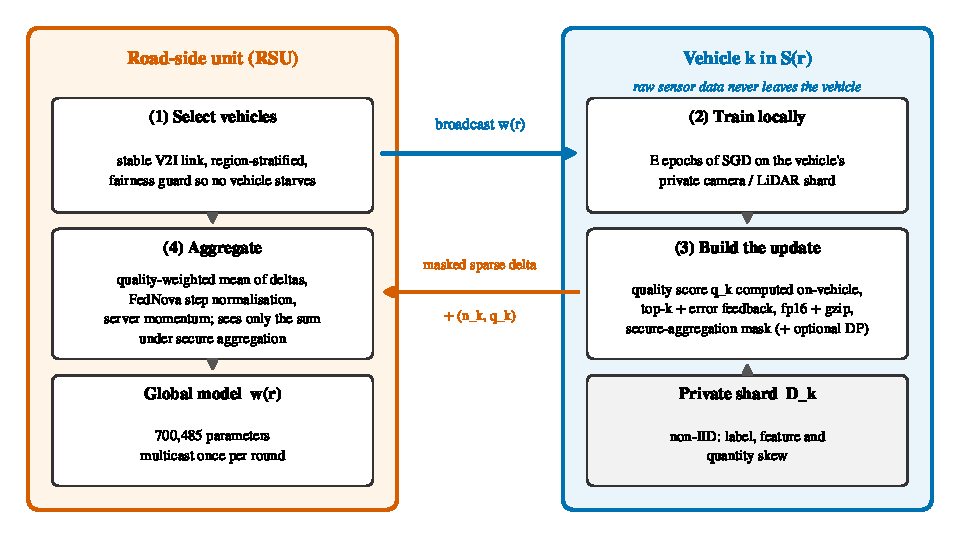
\includegraphics[width=0.86\textwidth]{fig1_architecture}
\caption{One federated round of FL-AV. The RSU selects vehicles (1) and multicasts the global model; each vehicle trains on its private shard (2), builds a compressed, masked update (3) and returns it; the RSU aggregates the quality-weighted deltas (4). Raw sensor data never leave the vehicle.}
\label{fig:arch}
\end{figure*}

\subsection{Quality-Aware Aggregation}\label{sec:quality}
Standard FedAvg weights vehicle $k$ by $n_k/n$. We instead use
\begin{equation}
\alpha_k=\frac{q_k\,n_k}{\sum_{j\in S(r)}q_j\,n_j},\qquad \sum_{k}\alpha_k=1,\quad \alpha_k\ge 0,
\label{eq:alpha}
\end{equation}
so the weights always lie on the probability simplex. The quality score is computed on the vehicle as
\begin{equation}
\begin{aligned}
q_k&=\clamp\!\big(\mathrm{sim}_k\cdot \mathrm{health}_k,\;q_{\min},\;q_{\max}\big),\\
\mathrm{sim}_k&=1-H(p_k,p_{\mathrm{ref}}),
\end{aligned}
\label{eq:quality}
\end{equation}
where $H(p,q)=\lVert\sqrt{p}-\sqrt{q}\rVert_2/\sqrt{2}\in[0,1]$ is the Hellinger distance between the vehicle's label histogram $p_k$ and a fleet reference histogram, and $\mathrm{health}_k$ is a sensor-health score built from blur, occlusion, rain intensity and a calibration flag, never from labels. A floor $q_{\min}=0.05$ keeps a rare but clean region contributing, so that a vehicle is strongly damped only when it is both off-distribution and degraded. The reference histogram is the one fleet-level statistic the scheme needs; in deployment it should itself be collected under secure aggregation.

\subsection{Normalised Averaging for Unequal Local Work}\label{sec:fednova}
When step counts $\tau_k$ differ, a plain weighted mean of deltas over-weights vehicles that took more steps. We use the FedNova aggregate~\cite{wang2020fednova}
\begin{equation}
\Delta=\Big(\sum_{k}\alpha_k\tau_k\Big)\sum_{k}\alpha_k\frac{\Delta W_k}{\tau_k},
\label{eq:fednova}
\end{equation}
which is inert when all $\tau_k$ are equal. Because quantity skew makes $\tau_k$ differ even with a fixed epoch count, the correction is not a corner case. However, our audit (Section~\ref{sec:audit}) found that on the secure-aggregation path, which is enabled by default, the normalised aggregate is overwritten by the raw weighted mean. The headline proposed arm therefore contains no normalisation effect; \eqref{eq:fednova} was exercised only in the non-secure ablation runs.

\subsection{Server Momentum}
The server smooths the aggregate with momentum $\beta$: $v\leftarrow\beta v+\Delta$ and $w^{(r+1)}=w^{(r)}+(1-\beta)v+\beta\Delta$. The convex blend makes the first round identical to plain FedAvg and lets later rounds inherit a smoothed direction~\cite{hsu2019noniid}.

\subsection{Connectivity- and Trajectory-Aware Selection}\label{sec:selection}
The selector fills $\lceil CN\rceil$ slots in four steps. (i) \emph{Connectivity filter:} vehicles whose predicted link uptime falls below 0.55 are ineligible; if too few remain, the threshold is relaxed geometrically rather than returning an empty round. (ii) \emph{Starvation promotion:} eligible vehicles unselected for more than $K=12$ rounds move to the front of the queue. (iii) \emph{Region stratification:} slots are filled round-robin over regions with the highest-scoring vehicle of each. (iv) \emph{Score fill:} any remaining slots go to the highest scores, where the score is the deterministic ranking $0.55\,u_k+0.25\,h_k+0.01\log(1+n_k)+0.10/(1+m_k)$ of link uptime $u_k$, sensor quality $h_k$, shard size and selection count $m_k$. Selection is therefore neither random nor independent of the data. Because the starvation guard considers only eligible vehicles, it does not bound the selection gap of low-uptime vehicles (Section~\ref{sec:audit}).

\subsection{Transport Stack}\label{sec:transport}
Each uplink passes through four stages. (a) The vehicle sends the delta rather than the weights. (b) Top-$k$ sparsification with error feedback~\cite{stich2018sparsified,karimireddy2019ef} transmits the $k$ largest-magnitude coordinates and keeps the remainder in an on-vehicle residual,
\begin{equation}
d_k^{r}=\Delta W_k^{r}+e_k^{r-1},\quad s_k^{r}=\topk_k\!\big(d_k^{r}\big),\quad e_k^{r}=d_k^{r}-s_k^{r},
\label{eq:ef}
\end{equation}
so no coordinate is discarded, only delayed. (c) The sparse delta is serialised in float16, gzip-compressed and protected by a CRC32 checksum. (d) The global model is multicast once per cell instead of unicast to each vehicle. A closed-loop controller raises the sparsity when a round exceeds the 9\,MB budget and relaxes it when there is headroom. The cost $C_{\mathrm{total}}=\sum_{r}\sum_{k\in S(r)}(C^{\uparrow}+C^{\downarrow})$ is measured from serialised byte counts, including TLS record overhead and dropped uplinks; TLS handshake bytes are not counted.

\subsection{Privacy Mechanisms}\label{sec:privacy}
\subsubsection{Secure aggregation (simulated)}
Each pair $(i,j)$ of participants expands a shared seed into a mask $m_{ij}$; vehicle $i$ adds $+m_{ij}$ if $j>i$ and $-m_{ij}$ otherwise, so that
\begin{equation}
\textstyle\sum_{k}\big(\alpha_k\Delta W_k+\mathrm{mask}_k\big)=\sum_{k}\alpha_k\Delta W_k ,
\label{eq:secagg}
\end{equation}
and the runner verifies this identity every round. The implementation reproduces the arithmetic of the protocol~\cite{bonawitz2017secagg}, not its security: masks are real-valued and seeded from the public configuration seed, there is no key exchange or dropout recovery, and per-update norms are revealed to set the mask scale. We treat it as a functional model, not as a privacy mechanism.

\subsubsection{Differential privacy (optional)}
Each delta is clipped to norm $C_{\mathrm{clip}}$ and perturbed with $\mathcal{N}(0,\sigma^2 I)$, $\sigma=zC_{\mathrm{clip}}$, where $z$ is calibrated by a R\'enyi-DP accountant for the subsampled Gaussian mechanism~\cite{mironov2019sgm} composed over $R$ rounds. Under secure aggregation each vehicle adds $\sigma/\sqrt{|S|}$ so that the aggregate noise is $\mathcal{N}(0,\sigma^2)$. This accounting is not an end-to-end guarantee: the accountant assumes Poisson sampling independent of the data, whereas selection here is deterministic and data-dependent; the noise is split over selected rather than reporting vehicles; and the data-dependent weights $\alpha_k$ are released. No DP-enabled training run is reported.

\subsubsection{Robust aggregation (optional)}
Updates whose norm exceeds three times the median are rejected and the rest are combined by a coordinate-wise weighted trimmed mean. This option is mutually exclusive with secure aggregation, which hides the per-client values a trimmed mean needs.

\begin{algorithm}[!t]
\caption{One FL-AV training run}\label{alg:flav}
\begin{algorithmic}[1]
\Require fleet $\{D_k\}_{k=1}^{N}$, fraction $C$, rounds $R$, epochs $E$, momentum $\beta$, tolerance $\epsilon$
\Ensure global model $w$
\State $w\gets w^{(0)}$, $v\gets 0$, $e_k\gets 0$ for all $k$
\For{$r=1,\dots,R$}
  \State $S\gets\textsc{Select}(C,\text{uptime},\text{regions},K)$ \Comment{Sec.~\ref{sec:selection}}
  \State multicast $w$ to all $k\in S$
  \ForAll{$k\in S$ \textbf{in parallel}}
    \State $w_k\gets\textsc{LocalSGD}(w,D_k,E)$;\; $\Delta W_k\gets w_k-w$
    \State $q_k\gets$ quality score \eqref{eq:quality}, computed on-vehicle
    \State $d_k\gets\Delta W_k+e_k$;\; $s_k\gets\topk(d_k)$;\; $e_k\gets d_k-s_k$
    \State send $\textsc{Mask}(\textsc{Encode}(s_k))$, $n_k$, $q_k$
  \EndFor
  \State $\alpha_k\gets q_k n_k/\sum_{j\in S}q_j n_j$ \Comment{\eqref{eq:alpha}}
  \State $\Delta\gets\textsc{SecureSum}(\{\alpha_k s_k\})$ \Comment{\eqref{eq:secagg}}
  \State $v\gets\beta v+\Delta$;\; $w_{\mathrm{new}}\gets w+(1-\beta)v+\beta\Delta$
  \If{$\lVert w_{\mathrm{new}}-w\rVert_2\le\epsilon$} \textbf{break} \EndIf
  \State $w\gets w_{\mathrm{new}}$
\EndFor
\end{algorithmic}
\end{algorithm}

Algorithm~\ref{alg:flav} summarises a run as shipped. Line~12 reflects the audit finding that the secure path applies the plain weighted sum rather than \eqref{eq:fednova}.

% =====================================================================
\section{Experimental Protocol}\label{sec:protocol}
\subsection{Data and Fleet}
Real driving datasets such as KITTI~\cite{geiger2012kitti} and nuScenes~\cite{caesar2020nuscenes} cannot be redistributed, and CARLA~\cite{dosovitskiy2017carla} requires a GPU simulator. We therefore use a CARLA-style procedural generator that reproduces the \emph{structure} of the problem rather than the appearance statistics of real sensors. Every cue a label depends on is drawn into the $32\times32$ image: object shape, aspect ratio and colour determine the class (six classes), the rendered rectangle is the box, and motion-streak length and direction plus lane-marking slant encode the six-waypoint trajectory. The fleet has $N=50$ vehicles with three combined skew axes: label skew $p_k\sim\mathrm{Dir}(0.4\cdot\mathbf{1})$; feature skew from region (urban, highway, rural) $\times$ weather (clear, rain, fog, night); and log-normal quantity skew ($\sigma=0.45$ around 220 samples; about 7\,700 training samples in total). About 12\% of vehicles are de-calibrated (extra blur, brightness drift and 25--45\% label corruption), which are precisely the vehicles $q_k$ is meant to discount. Each shard is split 70/15/15 into train, validation and test, and all arms are also scored on one IID global test set of 1\,800 samples covering every region--weather combination.

\subsection{Model}
The network is a MobileNetV3-style multi-task model~\cite{howard2019mobilenetv3} with 700\,485 parameters: a stem convolution, three stages of inverted residual blocks with squeeze-and-excitation, a $1\times1$ neck producing a $4\times4$ feature grid, and heads for class, box size, trajectory and a centre heat-map whose soft-argmax yields $(c_x,c_y)$. GroupNorm~\cite{wu2018groupnorm} is used throughout, because batch statistics are client-specific under non-IID data and averaging them is a known source of FedAvg divergence. The loss is $\mathrm{CE}+\lambda_{\mathrm{box}}[2\,\ell_{\mathrm{c}}+\ell_{\mathrm{s}}]+\lambda_{\mathrm{traj}}\ell_{\mathrm{t}}$ with Smooth-L1 terms $\ell$ for centre, size and trajectory, masked on background samples.

\subsection{Compared Arms}
All arms share one fleet and one seed (1337). \emph{Centralized} pools all raw data and is an upper bound that violates the privacy constraint. \emph{Local-only} trains each vehicle alone and is a lower bound. \emph{Standard FedAvg} uses $n_k/n$ weights, no momentum and fp32 full-weight unicast transfer with gzip; it uses the same score-ranked selector with the filter, stratification and starvation guard disabled, and is therefore \emph{not} uniform-random selection. \emph{Proposed} uses quality-aware weights, the full selector, server momentum, the full transport stack and secure aggregation, with adaptive local epochs disabled (Section~\ref{sec:ablation}). Common settings are $C=0.3$ (15 vehicles per round), $E=5$, $R_{\max}=60$, learning rate 0.01 with cosine decay, SGD momentum 0.9 and batch size 32; Appendix~\ref{app:hyper} lists all hyperparameters.

\subsection{Metrics}
\emph{Accuracy} is top-1 classification accuracy on the global test set. \emph{mAP@0.5} counts a detection as correct when the class matches and the box IoU is at least 0.5. \emph{ADE} is the average displacement error of the predicted trajectory. \emph{Dispersion} is the standard deviation and minimum of accuracy over the vehicles' local test splits. \emph{Communication} is measured from serialised bytes. The best round is selected on the global test set and is therefore optimistic; we use the \emph{mean of the last ten rounds} as the primary accuracy metric.

% =====================================================================
\section{Results}\label{sec:results}
All numbers are read from the committed artefacts in \code{results/} and are regenerated by \code{paper/make\_paper\_figures.py}. Unless stated otherwise they come from a single seed.

\subsection{Collaboration Recovers Most of the Centralized Ceiling}\label{sec:collab}
Table~\ref{tab:main} reports the main benchmark. Federation is worth 58 points over local-only training on the primary metric (82.94\% versus 24.70\%) and recovers 94.0\% of the centralized ceiling (82.94/88.21) without any raw sensor sample leaving a vehicle (Fig.~\ref{fig:curves}). Vehicles training alone cannot learn the six-class problem from skewed shards of about 150 training samples.

\begin{table}[!t]
\renewcommand{\arraystretch}{1.1}
\caption{Main Benchmark ($N=50$, $C=0.3$, $E=5$, $R=60$, $\alpha=0.4$, Seed 1337)}
\label{tab:main}
\centering
\footnotesize
\setlength{\tabcolsep}{3.2pt}
\begin{tabular}{@{}lrrrr@{}}
\toprule
Metric & Central. & Local & FedAvg & Proposed\\
\midrule
Acc., last-10 mean (\%) $\uparrow$ & 88.21 & 24.70 & 80.09 & \textbf{82.94}\\
Acc., best round (\%)$^{\dagger}$ $\uparrow$ & 89.89 & 25.19 & 83.00 & \textbf{84.67}\\
mAP@0.5 $\uparrow$ & 0.544 & 0.005 & 0.089 & \textbf{0.100}\\
Trajectory ADE $\downarrow$ & 0.188 & 0.323 & \textbf{0.197} & 0.202\\
MB per round $\downarrow$ & -- & 0 & 74.56 & \textbf{8.72}\\
Total MB, 60 rounds $\downarrow$ & 90.2$^{\ddagger}$ & 0 & 4\,473.7 & \textbf{523.3}\\
Client acc.\ std $\downarrow$ & 0.126 & 0.069$^{\S}$ & \textbf{0.130} & 0.137\\
Worst-client acc.\ $\uparrow$ & 0.509 & 0.169 & \textbf{0.463} & 0.327\\
Raw data leave vehicle & yes & no & no & no\\
\bottomrule
\end{tabular}
\vspace{2pt}

\parbox{\columnwidth}{\scriptsize Bold marks the better of the two federated arms. $^{\dagger}$Selected on the test set, hence optimistic. $^{\ddagger}$Raw-data upload. $^{\S}$Computed on a different test set; not comparable.}
\end{table}

\begin{figure}[!t]
\centering
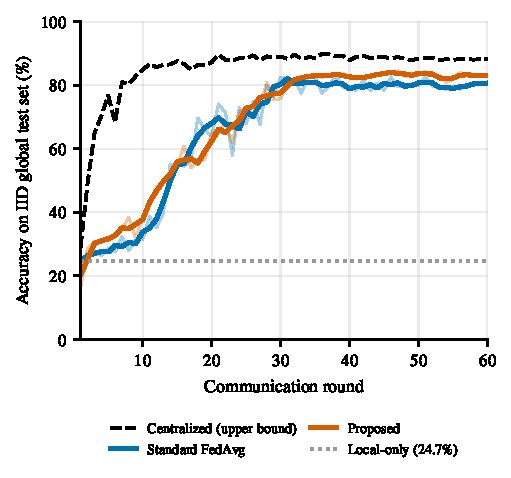
\includegraphics[width=\columnwidth]{fig2_learning_curves}
\caption{Accuracy on the IID global test set versus communication round. Thick lines are 3-round moving averages of the thin raw curves; the local-only arm is drawn as its last-10-round mean. One seed.}
\label{fig:curves}
\end{figure}

\subsection{Communication}\label{sec:comm}
The proposed stack transmits 8.72\,MB per round against 74.56\,MB for standard FedAvg, 523\,MB against 4\,474\,MB over 60 rounds ($-88.3\%$; Fig.~\ref{fig:comm}), and meets the 9\,MB budget. Measured in isolation on the same model and 15 vehicles, raw float32 unicast costs 80.2\,MB per round; gzip reduces this to 74.3\,MB, float16 to 37.1\,MB, top-25\% sparsity to 25.2\,MB and RSU multicast to 8.0\,MB (Fig.~\ref{fig:appC}b). The in-training figure is slightly higher because it includes TLS record overhead and dropped uplinks.

\begin{figure*}[!t]
\centering
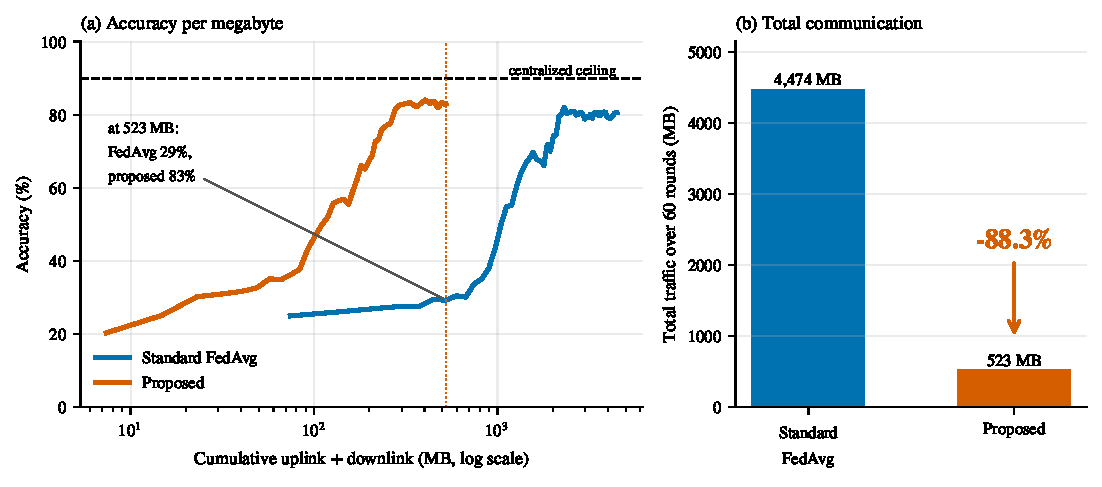
\includegraphics[width=0.92\textwidth]{fig3_communication}
\caption{Communication. (a) Accuracy versus cumulative traffic on a logarithmic axis: at 523\,MB the proposed run has finished at 83\% accuracy, whereas standard FedAvg is at 29\%. (b) Total traffic over 60 rounds. Panel (a) is largely a rescaling of Fig.~\ref{fig:curves} by the per-round cost; it shows that the accuracy curve is not shifted to later rounds.}
\label{fig:comm}
\end{figure*}

\subsubsection*{Attribution of the saving}
Of the 66.4\,MB per round saved beyond the gzip stage, float16 accounts for 56\% (37.3\,MB), multicast for 26\% (17.3\,MB) and top-$k$ sparsification with error feedback for only 18\% (11.8\,MB), because zeroed coordinates are gzip-coded rather than index-coded. About 82\% of the saving thus comes from engineering choices that any FedAvg deployment could adopt. No FedAvg baseline with the same transport was run, so the saving against a transport-matched baseline is untested and would be smaller; the headline figure holds for the stated baseline (fp32, full weights, unicast, gzip).

\subsubsection*{Accuracy cost}
In a controlled comparison at $R=30$ on identical algorithmic settings, adding compression and secure aggregation changed accuracy from 61.6\% to 60.9\% ($-0.7$ points) while traffic fell from 74.55 to 8.68\,MB per round. The two changes were introduced together and the difference is within single-seed noise, so we report it as no measurable loss.

\subsection{Convergence Speed}\label{sec:convergence}
Table~\ref{tab:conv} lists the first round at which each arm reaches a given accuracy. The proposed arm is faster to 60\% and 83\%, slower to 70\%, and tied elsewhere; the requirement of a 25\% reduction in rounds-to-target is not met (Table~\ref{tab:accept}). Over the final 20 rounds the proposed arm averages $83.1\pm0.9\%$ and FedAvg $80.0\pm1.3\%$ (mean $\pm$ standard deviation across rounds), and the proposed arm is higher in 28 of the last 30 rounds. Because rounds are strongly autocorrelated, these descriptive statistics do not constitute a significance test.

\begin{table}[!t]
\renewcommand{\arraystretch}{1.1}
\caption{First Round Reaching a Global Accuracy Threshold}
\label{tab:conv}
\centering
\footnotesize
\begin{tabular}{@{}lrrr@{}}
\toprule
Threshold & Centralized & Std.\ FedAvg & Proposed\\
\midrule
50\% & 3 & 14 & 14\\
60\% & 3 & 18 & \textbf{16}\\
70\% & 4 & \textbf{21} & 24\\
75\% & 5 & 28 & 28\\
80\% & 7 & 28 & 28\\
83\% & 10 & 38 & \textbf{34}\\
\bottomrule
\end{tabular}
\end{table}

\subsection{Single-Mechanism Ablation}\label{sec:ablation}
Each mechanism was run in isolation against a FedAvg control at $R=30$ on the same fleet and seed, with transport held constant (Table~\ref{tab:ablation}, Fig.~\ref{fig:ablation}). Two caveats apply: the control uses the same score-ranked selector as the FedAvg arm, so the selection effect is measured against a link-ranked rather than random baseline; and the code revision that produced each arm is not recorded, so arms may straddle the commit that introduced normalised averaging.

\begin{table*}[!t]
\renewcommand{\arraystretch}{1.1}
\caption{Single-Mechanism Ablation at $R=30$ (One Seed). Std Is the Cross-Client Accuracy Standard Deviation; Min Is the Worst Vehicle}
\label{tab:ablation}
\centering
\footnotesize
\begin{tabular}{@{}lrrrrr@{}}
\toprule
Arm & Accuracy (\%) & $\Delta$ vs.\ control (pts) & Std & Min & MB/round\\
\midrule
FedAvg control & 70.78 & -- & 0.154 & 0.224 & 74.55\\
+ Connectivity/trajectory-aware selection & 79.00 & \textbf{+8.2} & 0.124 & \textbf{0.429} & 74.56\\
+ Server momentum & 75.00 & +4.2 & 0.157 & 0.245 & 74.56\\
+ Quality-aware weighting & 72.78 & +2.0 & \textbf{0.106} & 0.388 & 74.56\\
+ Adaptive local epochs (plain mean) & 58.61 & $-12.2$ & 0.193 & 0.122 & 74.56\\
+ Adaptive local epochs (normalised averaging) & 64.56 & $-6.2$ & 0.141 & 0.224 & 74.55\\
All algorithmic, adaptive epochs on (plain mean) & 61.61 & $-9.2$ & 0.155 & 0.286 & 74.55\\
All algorithmic, adaptive epochs on (normalised) & 68.17 & $-2.6$ & 0.164 & 0.327 & 74.56\\
All algorithmic (plain) + compression + secure agg. & 60.89 & $-0.7^{\ast}$ & 0.165 & 0.245 & \textbf{8.68}\\
\bottomrule
\end{tabular}
\vspace{2pt}

\parbox{0.9\textwidth}{\centering\scriptsize $^{\ast}$Relative to the ``all algorithmic, plain mean'' arm, not to the FedAvg control.}
\end{table*}

\begin{figure*}[!t]
\centering
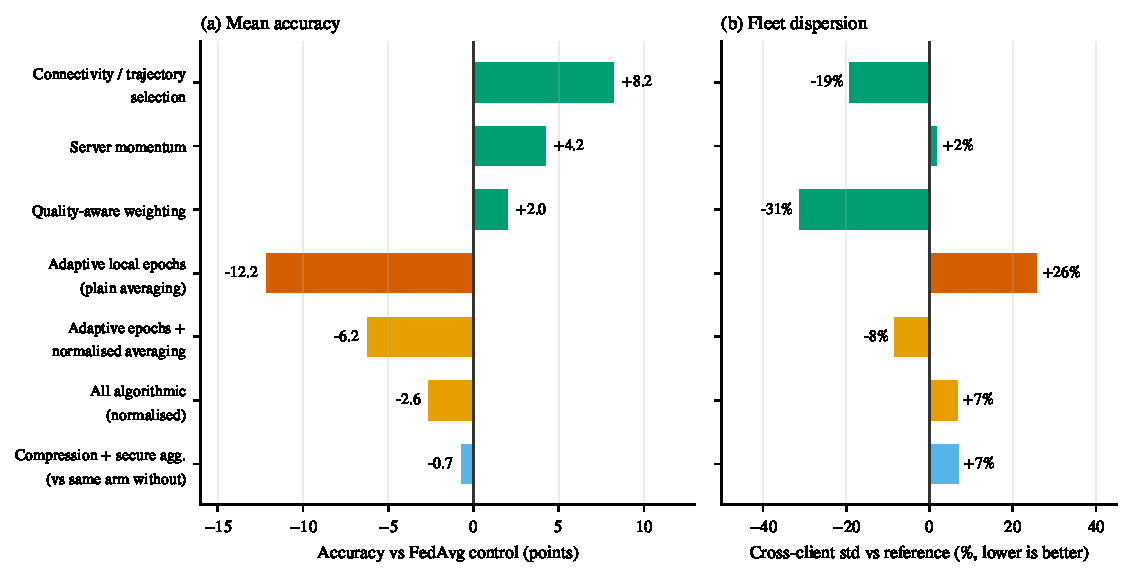
\includegraphics[width=0.92\textwidth]{fig4_ablation}
\caption{Change in (a) mean accuracy and (b) cross-client accuracy standard deviation relative to the FedAvg control (70.8\%, std 0.154), $R=30$, one seed. Green: mechanisms that help; red: the harmful mechanism; amber: its partial correction; blue: compression plus secure aggregation relative to the identical arm without them.}
\label{fig:ablation}
\end{figure*}

\subsubsection*{Selection, momentum and quality weighting each help}
Quality-aware weighting reduces the cross-client standard deviation by 31\%, the non-IID robustness it is designed to provide. The +8.2 points for selection is the largest single gain, but it is relative to a link-ranked control and combines three components that were not separated.

\subsubsection*{Adaptive local epochs are harmful}
Scaling the epoch count to on-board compute makes $\tau_k$ differ across vehicles. A vehicle that ran eight epochs contributes a longer vector than one that ran one, and a plain weighted mean over-weights the fast vehicles regardless of $\alpha_k$, so the aggregate converges to the wrong point (Fig.~\ref{fig:appC}a shows the bias growing linearly with the step-count ratio). Normalised averaging removes that bias and recovers about half of the loss ($-12.2$ to $-6.2$ alone; $-9.2$ to $-2.6$ combined). The remaining deficit is real and not yet explained. We therefore keep the mechanism implemented and tested but disabled by default.

\subsubsection*{The gains do not add}
The three helpful mechanisms (+8.2, +4.2 and +2.0 in isolation) combine to only +1.7 points (best round) in the 60-round benchmark, so they overlap or interfere. The ablation and benchmark also differ in horizon (30 versus 60 rounds); the interaction structure remains open.

\subsection{Tail Behaviour}\label{sec:tail}
The proposed arm raises mean per-vehicle accuracy slightly (79.4\% versus 78.5\%) but has higher dispersion (0.137 versus 0.130) and a lower worst-vehicle accuracy (32.7\% versus 46.3\%; Fig.~\ref{fig:tail}). In isolation quality weighting \emph{reduces} dispersion by 31\%, so something in the combined system reverses its effect. The project documentation attributes this to connectivity-aware selection seeing poorly connected vehicles less often. A selector-only simulation with the committed seed contradicts that explanation: the proposed selector chose the six vehicles with uptime below 0.55 on average 3.5 times in 60 rounds, the FedAvg selector 1.7 times, and uniform sampling would choose each vehicle 18 times. Both arms under-sample poorly connected vehicles, and the proposed arm does so less. The remaining candidates (quality weighting discounting de-calibrated vehicles in the tail, server momentum, the absence of normalised averaging on the secure path, and noisy local test splits) are untested, so the cause of the regression is unresolved.

\begin{figure*}[!t]
\centering
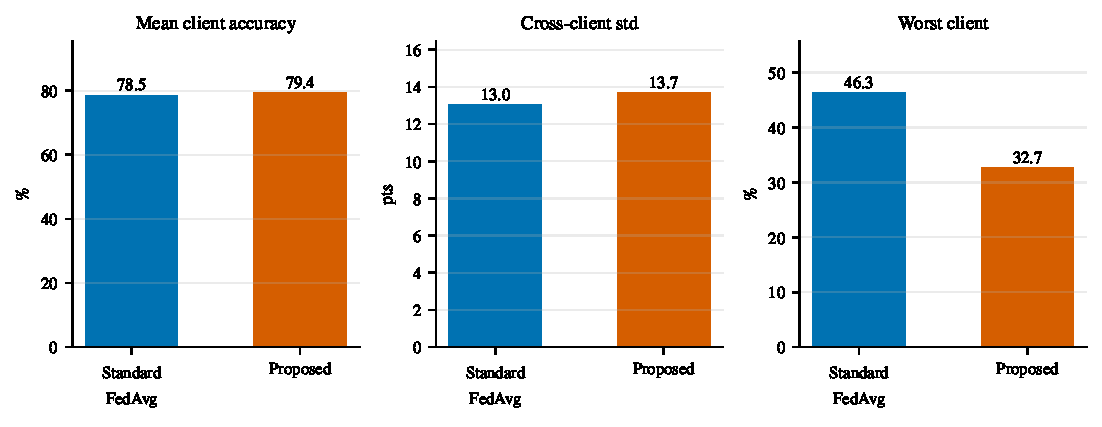
\includegraphics[width=0.78\textwidth]{fig5_tail}
\caption{Per-vehicle accuracy at round 60: fleet mean, cross-client standard deviation and worst vehicle, for standard FedAvg and the proposed arm. Each vehicle is scored on its own local test split.}
\label{fig:tail}
\end{figure*}

The worst-vehicle statistic must be read with care. The worst vehicles were scored on 41 to 49 local test samples, so a single vehicle's accuracy has a binomial standard error of about 7 points, and the minimum is the extreme of 50 such noisy values. The 13.6-point gap is about two standard errors of one vehicle's estimate. We report it because it is the least favourable number for the method and because its direction agrees with the dispersion statistic.

\subsection{Acceptance Audit}\label{sec:acceptance}
The project's requirements document defines eight acceptance criteria (Table~\ref{tab:accept}); five fail. The 90\% absolute target is a scale artefact, since the centralized upper bound on this data is 89.9\%; we report it as failed rather than redefine it.

\begin{table}[!t]
\renewcommand{\arraystretch}{1.1}
\caption{Acceptance Criteria From the Requirements Document}
\label{tab:accept}
\centering
\footnotesize
\setlength{\tabcolsep}{3pt}
\begin{tabular}{@{}L{2.0cm}L{2.6cm}L{1.9cm}c@{}}
\toprule
Criterion & Requirement & Observed & Result\\
\midrule
Accuracy & $\ge 90\%$ & 84.67\% & Fail\\
Speed-up & $\ge25\%$ fewer rounds than FedAvg & target not reached & Fail\\
Comm.\ saving & $\ge30\%$ less MB/round & $-88.3\%$ & Pass\\
Comm.\ budget & $\le 9.0$ MB/round & 8.72 & Pass\\
Non-IID robustness & dispersion $\le$ FedAvg & 0.137 vs.\ 0.130 & Fail\\
Relative speed-up & $\ge25\%$ fewer rounds to 95\% of centralized & not reached & Fail\\
Ceiling ratio & $\ge 95\%$ of centralized & 94.2\% & Fail\\
Privacy & no raw-data egress & none & Pass\\
\bottomrule
\end{tabular}
\end{table}

\subsection{Verification of the Mathematics}\label{sec:verify}
Every equation was checked numerically against the shipped implementation (14 verification figures; \code{docs/figures/residuals.json}). The maximum deviation of $\sum_k\alpha_k$ from one over 4\,000 draws is $5.6\times10^{-16}$. On a five-vehicle example, \eqref{eq:quality} reduces a degraded large shard's aggregation share from 35.7\% to 11.2\%. Over $\tau\in[1,12]$, \eqref{eq:fednova} matches the reference exactly, whereas the plain mean deviates by up to 8.25. For sampling rate 0.3, 60 rounds and $\delta=10^{-5}$, the calibrated multiplier $z=1.748$ yields $\varepsilon=7.996$ under the accountant's own assumptions, which, as noted in Section~\ref{sec:privacy}, do not hold for this selector. The error-feedback residual stays within its bound $((1-\delta)/\delta)\lVert u\rVert$, with relative error at round 60 of 6.8\%, 2.2\% and 0.9\% for keep ratios 0.1, 0.25 and 0.5. Against six sign-flipping clients out of 20, the plain mean's maximum error is 2.8 and the norm filter with trimmed mean's is zero.

The verification also exposed a defect. With float32 accumulation and unit mask scale, the relative error of the recovered sum in \eqref{eq:secagg} was 0.18 at 64 participants and exceeded the runner's tolerance of $10^{-3}$ from eight participants onward, because each client sums its pair masks in a different order and float32 addition is not associative. The shipped path uses float64 accumulation and masks scaled to the update, giving an error of $1.3\times10^{-7}$ at 64 participants while each masked update stays below a mask at least 57 times its magnitude (Fig.~\ref{fig:appC}c). The defect is fixed and covered by a regression test; unit tests at small participant counts had passed.

\subsection{Code Audit and Provenance}\label{sec:audit}
While preparing this paper we audited the implementation and the committed artefacts independently of the project documentation, including by executing the code. All 51 tests pass (35\,s on a CPU). The audit nevertheless found the issues in Table~\ref{tab:audit}, listed in descending order of consequence.

\begin{table*}[!t]
\renewcommand{\arraystretch}{1.15}
\caption{Findings of the Code Audit and Their Consequences}
\label{tab:audit}
\centering
\footnotesize
\begin{tabular}{@{}c L{8.4cm} L{7.6cm}@{}}
\toprule
\# & Finding & Consequence for this paper\\
\midrule
1 & \textbf{Mixed code revisions.} The committed FedAvg arm predates normalised averaging; at the current revision its configuration fingerprint would be \code{bf38429e1cff}, not the committed \code{6ce7acb93704}. The proposed arm was rerun twice. & The arms in Table~\ref{tab:main} were not generated by one revision, so their difference is not strictly attributable to the method.\\
2 & \textbf{Normalised averaging bypassed under secure aggregation}, which is on by default. A one-round test gives a difference of exactly 0 between normalisation on and off on the secure path, versus 4.6\% on the non-secure path. & The proposed arm contains no normalisation effect, and the $R=30$ correction cannot be transferred to the shipped configuration.\\
3 & \textbf{The FedAvg baseline is not random.} It uses the score-ranked selector (55\% weight on link uptime); selection Gini 0.538 versus about 0.11 for uniform sampling. & All arms and the ablation control are link-biased; the selection effect is measured against that control, and the documented tail explanation is contradicted.\\
4 & \textbf{The starvation guard does not bound gaps.} It considers only vehicles above the uptime threshold; 28 of 50 vehicles waited more than $K=12$ rounds, and the longest gap was 38. & The claim that no vehicle starves is unsupported; the corresponding test sets the threshold to zero.\\
5 & \textbf{Test-set selection.} Best round, checkpoint and rounds-to-target use the global test set; validation splits are unused. & Best-round numbers are optimistic; last-10-round means are used as the primary metric.\\
6 & \textbf{Transport attribution.} No transport-matched FedAvg baseline; fp16 and multicast give about 82\% of the saving; the bandwidth controller and straggler timeout never fired. & The 88.3\% figure is valid only against the stated baseline; the controller is unexercised.\\
7 & \textbf{Privacy.} Secure aggregation uses public-seed masks; the DP accountant's assumptions do not hold; no DP training run exists. & No claim of cryptographic security or end-to-end DP is made.\\
8 & \textbf{Metrics.} mAP@0.5 is a single-object proxy; ADE is in normalised synthetic units; local-only dispersion uses a different test set. & Detection and trajectory numbers are comparable between arms only.\\
\bottomrule
\end{tabular}
\end{table*}

\subsubsection*{What survives}
Findings 1--5 qualify the comparison of the proposed arm against FedAvg: the 1.7--2.9-point accuracy difference, the dispersion and tail numbers, and the selection effect. They do not affect the federation effect over local-only training and the 94\% ceiling recovery (an effect of more than 50 points), the mechanism and magnitude of the adaptive-epoch harm (which also rests on a closed-form micro-benchmark), the numerical verification, or the byte-exact traffic accounting for the stated baseline. No claim survives that the proposed arm beats FedAvg on mean accuracy, that selection caused a specific gain, that no vehicle starves, that normalised averaging was active in the headline run, or that the system provides cryptographic or end-to-end differential privacy.

\subsubsection*{Corrective plan}
(a) Regenerate every arm from one revision with the defects fixed: normalisation on the secure path, a uniform-random baseline selector and a starvation guard over all vehicles. (b) Add a transport-matched FedAvg baseline. (c) Select checkpoints on per-vehicle validation data. (d) Run at least ten seeds and report bootstrap confidence intervals~\cite{agarwal2021precipice}. (e) Add FedProx~\cite{li2020fedprox} and SCAFFOLD~\cite{karimireddy2020scaffold} baselines. Until this is done, the present results should be read as a verified account of what the evidence does and does not show rather than as a final evaluation.

% =====================================================================
\section{Discussion}\label{sec:discussion}
\subsubsection*{What the evidence supports}
Three findings are large relative to any plausible single-seed noise. Federation recovers most of the value of pooling (+58 points over local-only). Against an uncompressed unicast baseline the transport stack removes almost nine tenths of the traffic without measurable accuracy loss, although most of that saving is due to precision and multicast. Adaptive local epochs with plain averaging are harmful, and the mechanism is identified and verified in a closed-form micro-benchmark.

\subsubsection*{What it does not support}
The 1.7--2.9-point advantage over FedAvg and the ordering of the three mildly helpful mechanisms lie within single-seed variability and are qualified by the audit. Faster convergence, better tail behaviour and better localisation are not claimed.

\subsubsection*{Why mAP stays low}
All federated arms reach mAP@0.5 of only 0.09--0.10 against 0.54 for the centralized arm, although classification accuracy is close. Localisation appears to be the first capability that non-IID averaging degrades, plausibly because box regression depends on spatial features that differ by region and weather. This is the most informative gap for future work and the strongest argument against presenting the system as deployable.

\subsection{Threats to Validity}\label{sec:limits}
\emph{Statistical:} one seed and one fleet draw; differences of one to three points cannot be ranked. \emph{External:} the data are synthetic, so absolute accuracies are not comparable with KITTI or nuScenes results, and the scale is small (about 7\,700 samples, $32\times32$ images, 0.7\,M parameters); the percentage traffic reduction is the transferable quantity. \emph{Construct:} V2I is parametric; secure aggregation is a functional simulation; DP is verified only at the accountant level under unmet assumptions; the Byzantine defence is verified only in a micro-benchmark; FedAvg is the only federated baseline. \emph{Internal:} the audit findings of Table~\ref{tab:audit}. \emph{Leakage:} the similarity score requires a fleet reference histogram, which should be collected under secure aggregation in deployment.

\subsection{Ethics and Broader Impact}
The study uses no human subjects, real vehicle data or personal information. Federated training reduces the movement of raw sensor data but is not by itself a privacy guarantee, since deltas can leak information~\cite{zhu2019dlg}; no configuration here is private in the formal sense. Perception models for driving are safety-critical, and the tail behaviour of Section~\ref{sec:tail} means that average accuracy must never be used as evidence of safety. Any deployment would require validation far beyond this simulation.

% =====================================================================
\section{Conclusion}\label{sec:conclusion}
We built and measured a federated-learning framework for collaborative autonomous-vehicle perception. Relative to an uncompressed baseline, its transport stack removed 88.3\% of the traffic, mostly through precision and multicast, without measurable accuracy loss; federation recovered 94\% of the centralized ceiling without sharing raw data; and a controlled ablation identified adaptive local epochs as clearly harmful and explained why. The framework did not accelerate convergence, did not improve the worst-served vehicle and leaves detection quality far below the centralized bound. An audit of our own code and artefacts found defects that qualify the comparison against FedAvg, which we report together with a corrective plan. We offer the results as a candid baseline, together with the code, configurations and committed artefacts needed to replicate or refute them.

% =====================================================================
\appendices

\section{Claim--Evidence Map}\label{app:claims}
Table~\ref{tab:claims} maps each quantitative claim to its source artefact. \emph{Robust}: large relative to single-seed noise. \emph{Indicative}: direction probably right, magnitude not established. \emph{Verified}: checked against a closed form.

\begin{table*}[!t]
\renewcommand{\arraystretch}{1.08}
\caption{Claims, Supporting Artefacts and Strength of Evidence}
\label{tab:claims}
\centering
\footnotesize
\begin{tabular}{@{}L{7.2cm}L{5.6cm}L{3.6cm}@{}}
\toprule
Claim & Evidence & Strength\\
\midrule
Federation gives about +58 points over local-only & \code{results/benchmark/} & Robust\\
Proposed reaches 94\% of centralized & same & Robust\\
Traffic $-88.3\%$ vs.\ fp32 unicast gzip baseline & same, serialised bytes & Robust for that baseline\\
fp16 and multicast give about 82\% of the saving & \code{docs/figures/residuals.json} & Verified (isolated)\\
Compression + secure aggregation cost 0.7 points & \code{results/attribution/} & Indicative, confounded\\
Proposed beats FedAvg by 1.7--2.9 points & benchmark & Weak (audit 1--3, 5)\\
Selection +8.2, momentum +4.2, quality +2.0 & \code{results/ingredients/} & Indicative\\
Quality weighting $-31\%$ dispersion & same & Indicative\\
Adaptive epochs $-12.2$ points & same & Robust\\
Normalised averaging recovers about half & \code{results/fix/fix.json} & Indicative\\
Mechanism of adaptive-epoch harm & verification figure, \code{residuals.json} & Verified\\
Normalised averaging active in headline run & -- & False (audit 2)\\
No vehicle starves & -- & False (audit 4)\\
Worst vehicle 32.7\% vs.\ 46.3\%; dispersion higher & benchmark & Weak (small test splits)\\
Cause of tail regression & -- & Unresolved\\
Secure-aggregation arithmetic exact; defect fixed & verification figure, tests & Verified (simulation)\\
Cryptographic security; DP guarantee; DP and Byzantine results in training & -- & No claim\\
\bottomrule
\end{tabular}
\end{table*}

\section{Hyperparameters}\label{app:hyper}
\begin{table}[!t]
\renewcommand{\arraystretch}{1.05}
\caption{Hyperparameters of All Federated Arms}
\label{tab:hyper}
\centering
\footnotesize
\begin{tabular}{@{}ll@{}}
\toprule
Setting & Value\\
\midrule
Clients $N$ / fraction $C$ / seed & 50 / 0.3 / 1337\\
Classes / image size / horizon & 6 / $32\times32$ / 6 waypoints\\
Samples per client / quantity $\sigma$ & 220 / 0.45\\
Dirichlet $\alpha$ / split & 0.4 / 70--15--15\\
Global test set / de-calibrated share & 1\,800 / $\approx$12\%\\
Parameters / embedding / dropout & 700\,485 / 192 / 0.05\\
Loss weights & $\lambda_{\mathrm{box}}=1$, $\lambda_{\mathrm{traj}}=0.5$\\
Rounds / local epochs / learning rate & 60 / 5 / 0.01 (cosine)\\
SGD momentum / batch / weight decay & 0.9 / 32 / $5\times10^{-4}$\\
Gradient clip / tolerance $\epsilon$ & 5.0 / $10^{-3}$\\
Uptime threshold / $K$ / timeout & 0.55 / 12 / 45\,s\\
Server momentum $\beta$ / $q_{\min}$ / $q_{\max}$ & 0.9 / 0.05 / 1.0\\
Adaptive epochs / Byzantine-robust & off / off\\
fp16 / gzip level / top-$k$ ratio & on / 6 / 0.25\\
Byte budget per round & 9\,MB\\
Secure aggregation / DP & on / off\\
DP budget when enabled & $(8,10^{-5})$, clip 1.0\\
\bottomrule
\end{tabular}
\end{table}

\section{Additional Verification Figures}\label{app:verify}
\begin{figure*}[!t]
\centering
\begin{minipage}[t]{0.325\textwidth}\centering
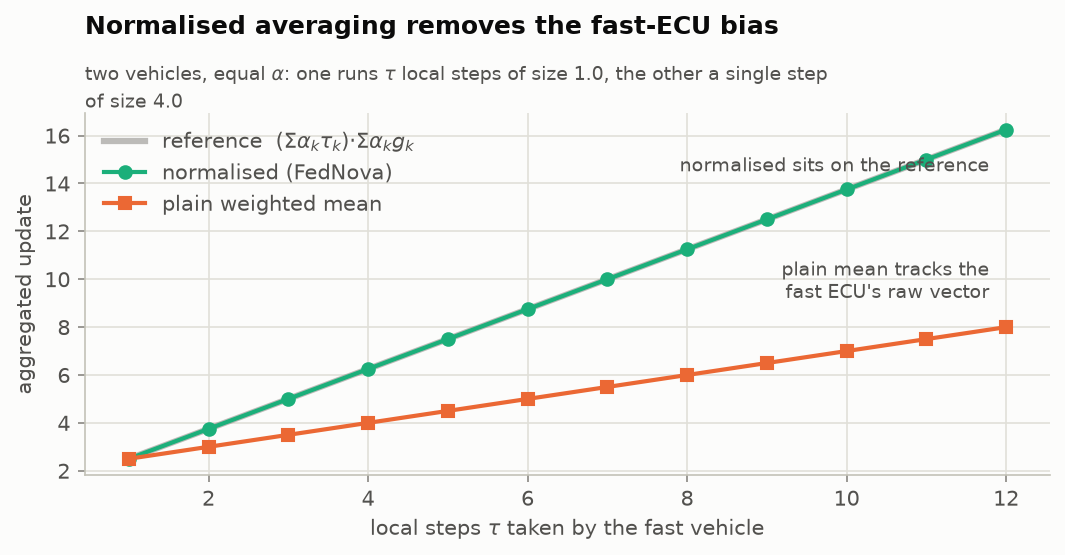
\includegraphics[width=\linewidth]{figC1_fednova}\\[-1pt]
{\footnotesize (a)}
\end{minipage}\hfill
\begin{minipage}[t]{0.325\textwidth}\centering
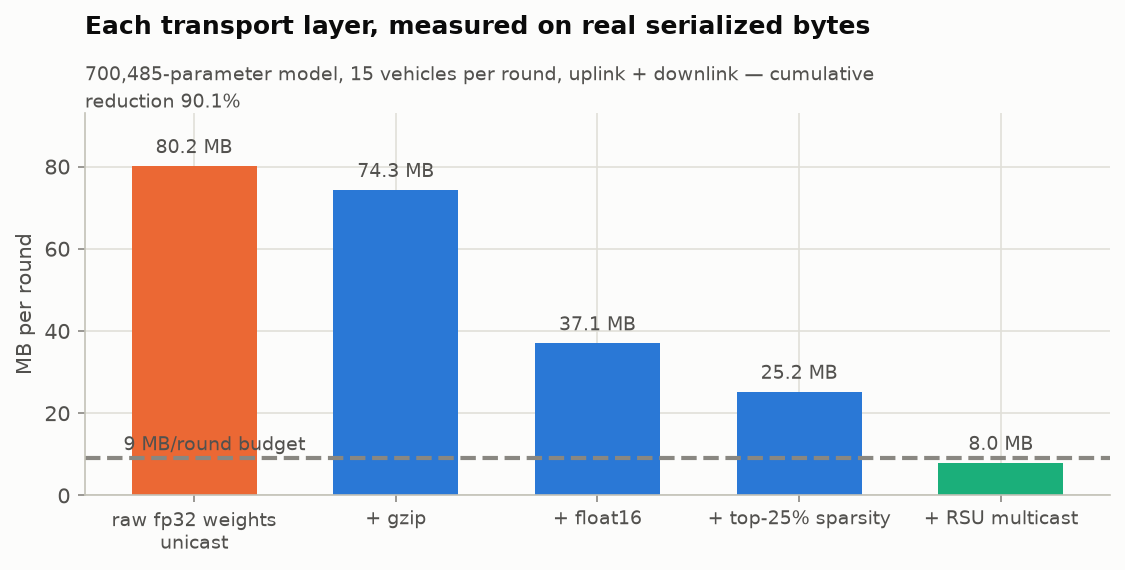
\includegraphics[width=\linewidth]{figC2_comm_stack}\\[-1pt]
{\footnotesize (b)}
\end{minipage}\hfill
\begin{minipage}[t]{0.325\textwidth}\centering
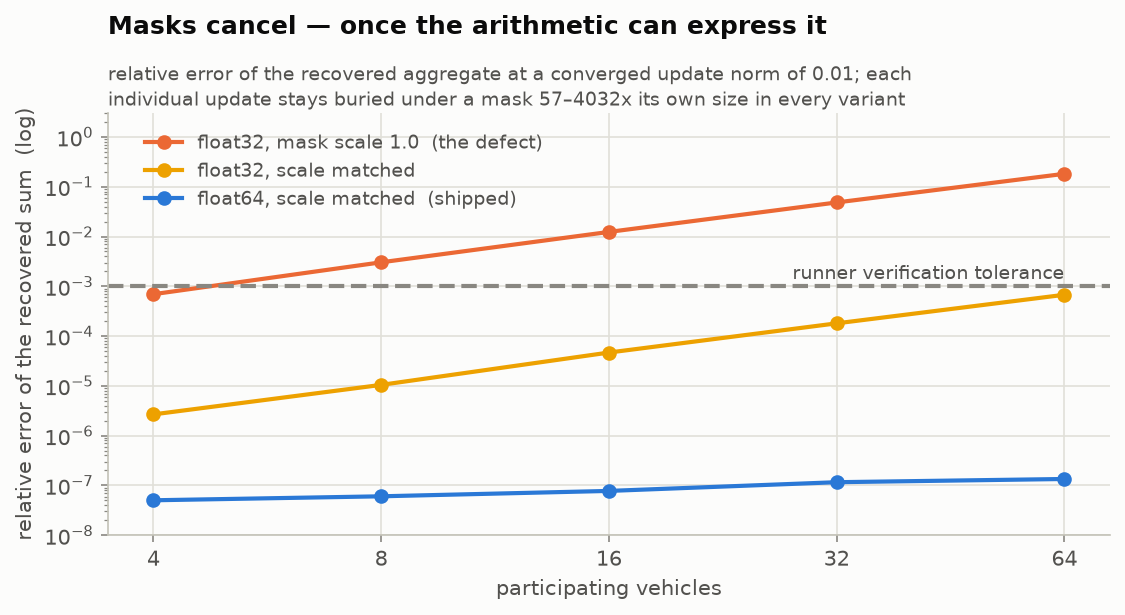
\includegraphics[width=\linewidth]{figC3_secure_agg}\\[-1pt]
{\footnotesize (c)}
\end{minipage}
\caption{Verification against closed forms. (a) Normalised averaging removes the fast-vehicle bias: with two equally weighted vehicles, the plain mean tracks the fast vehicle's raw vector while the normalised aggregate stays on the reference. (b) Contribution of each transport layer to per-round traffic for the 700\,485-parameter model and 15 vehicles. (c) Relative error of the recovered secure-aggregation sum for float32 with unit mask scale (the defect), float32 with matched scale, and float64 with matched scale (shipped).}
\label{fig:appC}
\end{figure*}

Fig.~\ref{fig:appC} reproduces three of the 14 verification figures generated by \code{scripts/make\_proof\_figures.py}.

\section{Reproduction}\label{app:repro}
The committed artefacts in \code{results/} are the runs reported here. Because they were not all produced by one code revision (Section~\ref{sec:audit}), a fresh benchmark at the current revision will differ from the committed FedAvg arm. The commands are:
\begin{itemize}
\item \code{python -m pytest tests/} (51 unit and mathematical tests);
\item \code{python -m fedav.cli benchmark -{}-config configs/default.yaml};
\item \code{python scripts/make\_proof\_figures.py};
\item \code{python paper/make\_paper\_figures.py --ieee}.
\end{itemize}
The proposed arm takes about one hour on four CPU cores.

\section*{Declarations}
\emph{Data and code availability:} data are generated by the included procedural generator from the configured seed; no external dataset is used. [Repository URL, licence and archival DOI to be added.] \emph{Competing interests:} [To be completed; any planned, pending or issued patent covering this work must be declared.] \emph{Funding:} [To be completed.] \emph{Author contributions:} [To be completed.] \emph{Use of AI assistance:} [To be described as required by the target venue.]

\balance
\bibliographystyle{IEEEtran}
\bibliography{refs}

\end{document}
